\documentclass[11pt]{article}

\usepackage[margin=1in]{geometry}
\usepackage[utf8]{inputenc}
\usepackage[T1]{fontenc}
\usepackage{newtxtext,newtxmath}
\usepackage{microtype}
\usepackage{graphicx}
\usepackage{booktabs}
\usepackage{multirow}
\usepackage{amsmath}
\usepackage{xcolor}
\usepackage[numbers,sort&compress]{natbib}
\usepackage{tikz}
\usetikzlibrary{arrows.meta,positioning,shapes.geometric,fit,backgrounds,calc}
\usepackage{pgfplots}
\pgfplotsset{compat=1.17}
\usepackage{algorithm}
\usepackage{algpseudocode}
\usepackage[colorlinks=true,linkcolor=blue!60!black,citecolor=blue!60!black,urlcolor=blue!60!black]{hyperref}
\usepackage[capitalise]{cleveref}
\usepackage{caption}
\captionsetup{font=small,labelfont=bf}

\definecolor{adblue}{HTML}{1F6FEB}
\definecolor{adgreen}{HTML}{3FB950}
\definecolor{adorange}{HTML}{D29922}
\definecolor{adred}{HTML}{CF222E}
\definecolor{adgray}{HTML}{57606A}

\newcommand{\evolve}{\texttt{evolve()}}
\newcommand{\code}[1]{\texttt{#1}}
\newcommand{\plugtitle}[1]{\textbf{\footnotesize #1}}
\newcommand{\Dval}{D_{\mathrm{val}}}

\title{\textbf{AgentDescent: Gradient Descent Where the Parameters Are Agents} \\[4pt]
\large A Parallel, Asynchronous, Merge-Based Framework for Self-Evolving Agent Artifacts}

\author{
  Birfy Chen\\
  \texttt{birfychen@gmail.com}\\[2pt]
  \small\url{https://github.com/Birfy/agentdescent}
}

\date{August 2026}

\begin{document}
\maketitle

\begin{abstract}
Self-improving agent systems evolve their own skills, prompts, and harnesses, but almost universally through a \emph{serial} loop --- one candidate proposed, evaluated, and accepted or rejected per iteration --- bounding improvement throughput at $O(1/T_{\mathrm{iter}})$. We present \textbf{AgentDescent}, a framework that transplants the distributed-training stack onto agent self-evolution: artifacts play the role of parameters, diffs with attached evidence play the role of gradients, a version-vectored ledger plays the role of the parameter server, and the optimizer step is a merge decision. Because diffs, unlike gradients, do not add, aggregation is performed as a discrete-space optimization: conflict resolution, fusion, and statistical acceptance under a per-artifact Beta posterior. We analyze efficiency as three composable sources of speedup: (i) overlap of I/O-bound rollouts, (ii) barrier-free asynchronous execution under per-diff bounded staleness, and (iii) \emph{reduced validation cost} --- held-out evaluation dominates the critical path, and merging $N$ concurrent proposals requires a single acceptance test, a saving that \emph{reflective merge} extends to artifacts whose proposals conflict. Eighteen published self-evolution algorithms are ported to the engine as plug-ins rather than forks and run unchanged under serial, synchronous, and asynchronous scheduling. On live models, removing the round barrier raises effective concurrency from $1.85\times$ to $3.22\times$ over a faithful serial control at a pinned budget; merged validation reduces model calls by 28\%; and all ported algorithms retain their learning behavior under the most aggressive schedule. An equal-budget comparison of merge-of-$N$ against best-of-$N$ selection does not yet separate the two, and we analyze why. Code and reproduction commands for every reported number are open source.
\end{abstract}

\section{Introduction}
\label{sec:intro}

A growing body of work shows that large-language-model agents can improve their own artifacts: prompts \citep{fernando2023promptbreeder,agrawal2025gepa}, in-context playbooks \citep{zhang2025ace}, skill libraries \citep{wang2023voyager,zheng2025skillweaver}, agentic workflows \citep{zhang2024aflow,hu2024adas}, and their own code \citep{zhang2025dgm,robeyns2025sica,yin2024godel,novikov2025alphaevolve}. These systems largely share an execution structure inherited from the G\"odel machine \citep{schmidhuber2003godel}: a serial improvement loop in which one candidate modification is proposed, evaluated, and accepted or rejected before the next is considered. If one iteration takes $T_{\mathrm{iter}}$ wall-clock seconds, improvement throughput is bounded at one accepted change per $T_{\mathrm{iter}}$, independent of available compute.

Distributed deep learning encountered the same bottleneck and resolved it with a now-standard stack: data-parallel workers computing gradients concurrently, parameter servers aggregating them \citep{li2014parameterserver}, staleness-tolerant asynchronous updates \citep{niu2011hogwild}, per-parameter adaptive steps \citep{kingma2014adam}, and gradient surgery for conflicting updates \citep{yu2020pcgrad}. This paper develops the thesis that the same stack, suitably reinterpreted, applies to agent self-evolution --- and identifies precisely where the reinterpretation must depart from the original.

\textbf{AgentDescent} (\cref{fig:architecture}) instantiates the mapping. A library of evolvable artifacts plays the role of the parameter tensor; a diff annotated with an \emph{evidence card} (the rollout that motivated it) plays the role of a gradient; a git-backed, version-vectored ledger plays the role of the parameter server; and the optimizer step is an \emph{aggregator} that merges concurrent diffs. $N$ workers roll out tasks against snapshots of the library and propose diffs in parallel; an asynchronous merger aggregates them, targeting $O(N/T_{\mathrm{iter}})$ improvement throughput.

The mapping is productive precisely because of where it breaks. \emph{Gradients add; diffs do not.} Two gradients can always be summed; two textual edits to the same artifact may be complementary, redundant, or contradictory. Aggregation is therefore not averaging but a decision procedure --- staleness filtering, conflict resolution, fusion, and a statistical acceptance test (\cref{sec:aggregator}). A second disanalogy is equally consequential: training code is not modifiable by the gradients it computes, whereas a self-evolving system can in principle rewrite its own verifier. AgentDescent therefore enforces a layered governance model in which safety-critical components are frozen (\cref{sec:governance}).

\paragraph{Contributions.}
\begin{enumerate}
  \item \textbf{A system design and a discrete-space aggregator} mapping the distributed-training stack onto parallel self-evolution --- per-diff bounded staleness, conflict projection, fusion, Beta-posterior acceptance, dual-branch promotion --- with a formal account of where the analogy holds and where it must break (\cref{sec:design,sec:aggregator}).
  \item \textbf{An efficiency analysis identifying three composable sources of speedup} (\cref{sec:efficiency}): rollout overlap, barrier removal, and --- specific to merge-based evolution --- reduced validation cost, in which merging collapses $N$ acceptance tests into one and \emph{reflective merge} extends the reduction to artifacts whose concurrent proposals conflict.
  \item \textbf{An extensibility mechanism} under which published algorithms are ported as plug-ins rather than forks (\cref{sec:pluggable,sec:ports}): a diff-encoding \code{strategy} plus an optional \code{aggregator\_factory}, or a declarative policy bundle. Eighteen ports run under all three schedulers without modification.
  \item \textbf{A live-model evaluation} (\cref{sec:experiments}): $1.85\times \to 3.22\times$ effective concurrency from barrier removal against a faithful serial control at a pinned budget; $28\%$ fewer model calls from merged validation; an eleven-algorithm scheduler study; evidence that quality is preserved under the most aggressive schedule; and an equal-budget merge-versus-selection comparison reported, with analysis, as not yet statistically separated.
\end{enumerate}

\section{Related Work}
\label{sec:related}

Self-evolving agents span prompt evolution \citep{fernando2023promptbreeder,agrawal2025gepa}, context and playbook evolution \citep{zhang2025ace}, skill libraries \citep{wang2023voyager,zheng2025skillweaver}, workflow and harness search \citep{zhang2024aflow,hu2024adas}, self-modifying code \citep{zhang2025dgm,robeyns2025sica,yin2024godel}, evolutionary program search \citep{novikov2025alphaevolve,openevolve2025,mouret2015mapelites}, and label-free self-play \citep{zhao2025absolutezero,huang2025rzero,xue2025agent0}, with reflection \citep{madaan2023selfrefine,shinn2023reflexion} as a shared inner proposal mechanism. Nearly all publish a serial outer loop; AgentDescent treats that loop as one scheduling regime among three. On the systems side, AgentDescent borrows its vocabulary from distributed training: parameter servers \citep{li2014parameterserver}, lock-free and bounded-staleness asynchrony \citep{niu2011hogwild,fu2025areal,roll2025flash}, per-parameter adaptivity \citep{kingma2014adam}, gradient surgery \citep{yu2020pcgrad}, weight averaging \citep{wortsman2022modelsoups}, and tensor/pipeline parallelism \citep{shoeybi2019megatron,huang2019gpipe}. Concurrent work on parallel self-evolution (barrier-free evolution loops; co-evolutionary verification \citep{coevoskills2026}) indicates that the throughput premise is an open hypothesis; our contribution is the specific synthesis --- concurrent, staleness-bounded, conflict-resolved diff-level merge over a versioned ledger --- together with the measurement harness required to evaluate it.

\section{Problem Setup and System Design}
\label{sec:design}

\subsection{Problem formulation}
\label{sec:setup}
Let $\mathcal{A}$ denote the space of \emph{artifact libraries}: finite keyed collections $A = \{a_k\}$ of versioned textual or executable artifacts (skills, prompts, playbooks, harness modules, file trees). An agent parameterized by $A$ induces a policy $\pi_A$; given a task distribution $\mathcal{D}$ and a bounded reward $r \in [0,1]$, the objective is
\begin{equation}
\label{eq:objective}
A^\star \;=\; \operatorname*{arg\,max}_{A \in \mathcal{A}} \; \mathbb{E}_{x \sim \mathcal{D}}\!\left[\, r\!\left(\pi_A(x),\, x\right) \right],
\end{equation}
optimized from rollout evidence only: $\mathcal{A}$ is discrete, and no gradient of $r$ with respect to $A$ exists. The serial baseline --- propose one candidate $A'$, evaluate on a held-out split $\Dval$, accept if better --- performs one accepted modification per iteration time $T_{\mathrm{iter}}$. AgentDescent's premise is that with $N$ concurrent proposers and merge-based aggregation, accepted-modification throughput can approach $O(N/T_{\mathrm{iter}})$ without sacrificing the acceptance discipline.

A \emph{diff} $d$ is a keyed partial edit over $A$, produced from a rollout by a \emph{strategy} $S$ that maps a natural-language proposal to operations on keys (rule slots, playbook bullets, file paths). The key structure is what makes two diffs comparable: edits on disjoint keys \emph{fuse}; edits on the same key \emph{conflict}. Every diff carries an \emph{evidence card} $e = (x, \tau, r, v_{\mathrm{base}})$ recording the task, rollout, reward, and the library version the proposer observed.

\begin{table}[t]
\centering
\small
\caption{The correspondence between distributed training and AgentDescent. The final row is a deliberate disanalogy, enforced rather than elided.}
\label{tab:analogy}
\begin{tabular}{@{}ll@{}}
\toprule
\textbf{Model training} & \textbf{AgentDescent} \\
\midrule
parameter tensor $\theta$ & library of \code{Evolvable} artifacts \\
gradient $g$ & \code{Diff} + \code{EvidenceCard} \\
parameter server & git-backed, version-vectored \code{Ledger} \\
optimizer step & \code{Aggregator} merge decision \\
per-parameter adaptive step (Adam) & per-artifact Beta-posterior acceptance \\
bounded staleness (async SGD/RL) & per-diff lag $\eta$ + rebase re-verification \\
EMA / weight averaging & \code{dev}/\code{stable} dual branch \\
training code (not self-modifiable) & L0 frozen governance layer \\
\bottomrule
\end{tabular}
\end{table}

\begin{figure}[t]
\centering
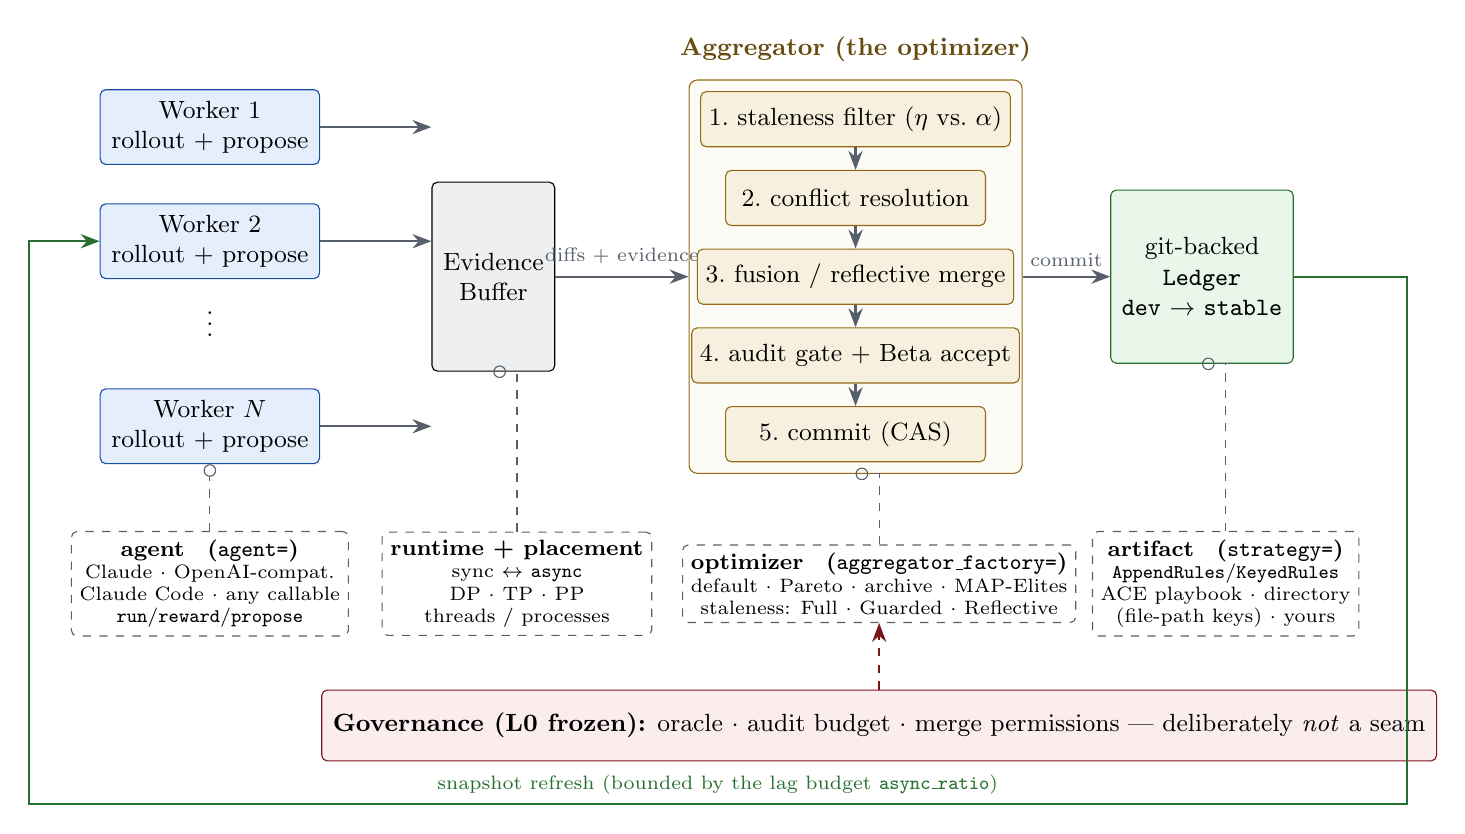
\begin{tikzpicture}[
  font=\small,
  box/.style={draw, rounded corners=2pt, align=center, minimum height=9mm, inner sep=4pt},
  worker/.style={box, fill=adblue!12, draw=adblue!70!black, minimum width=26mm},
  agg/.style={box, fill=adorange!15, draw=adorange!70!black, minimum width=33mm, minimum height=7mm, inner sep=3pt},
  ledger/.style={box, fill=adgreen!12, draw=adgreen!60!black},
  gov/.style={box, fill=adred!8, draw=adred!60!black},
  arr/.style={-{Stealth[length=2.4mm]}, thick, adgray},
  plug/.style={draw=adgray, dashed, rounded corners=2pt, align=center, font=\scriptsize, inner sep=3pt, fill=white},
  plugarr/.style={dashed, adgray, -{Circle[open, length=1.6mm]}},
]
% column 1: workers
\node[worker] (w1) at (0, 1.9)  {Worker 1\\rollout + propose};
\node[worker] (w2) at (0, 0.45) {Worker 2\\rollout + propose};
\node          at (0,-0.5) {$\vdots$};
\node[worker] (wn) at (0,-1.9)  {Worker $N$\\rollout + propose};

% column 2: evidence buffer
\node[box, fill=adgray!10, minimum height=24mm] (buf) at (3.6, 0) {Evidence\\Buffer};

% column 3: aggregator pipeline (top to bottom)
\node[agg] (stale)  at (8.2, 2.0)  {1.\ staleness filter ($\eta$ vs.\ $\alpha$)};
\node[agg] (conf)   at (8.2, 1.0)  {2.\ conflict resolution};
\node[agg] (fuse)   at (8.2, 0.0)  {3.\ fusion / reflective merge};
\node[agg] (gate)   at (8.2,-1.0)  {4.\ audit gate + Beta accept};
\node[agg] (commit) at (8.2,-2.0)  {5.\ commit (CAS)};
\begin{scope}[on background layer]
\node[draw=adorange!70!black, rounded corners=3pt, fit=(stale)(commit), inner sep=4pt, fill=adorange!4] (aggbox) {};
\end{scope}
\node[above=1mm of aggbox, adorange!50!black, font=\small\bfseries] {Aggregator (the optimizer)};

% column 4: ledger
\node[ledger, minimum height=22mm] (led) at (12.6, 0) {git-backed\\\code{Ledger}\\\code{dev} $\to$ \code{stable}};

% forward flow, left to right
\draw[arr] (w1.east) -- (buf.west |- w1.east);
\draw[arr] (w2.east) -- (buf.west |- w2.east);
\draw[arr] (wn.east) -- (buf.west |- wn.east);
\draw[arr] (buf.east) -- (aggbox.west) node[midway, above=1pt, font=\scriptsize] {diffs + evidence};
\draw[arr] (stale) -- (conf);
\draw[arr] (conf) -- (fuse);
\draw[arr] (fuse) -- (gate);
\draw[arr] (gate) -- (commit);
\draw[arr] (aggbox.east) -- (led.west) node[midway, above, font=\scriptsize] {commit};

% ---- pluggable-seam shelf: every dashed socket is one keyword argument ----
\node[plug] (pagent) at (0,-3.9) {\plugtitle{agent \, (\code{agent=})}\\Claude $\cdot$ OpenAI-compat.\\Claude Code $\cdot$ any callable\\\code{run}/\code{reward}/\code{propose}};
\node[plug] (prun)   at (3.9,-3.9) {\plugtitle{runtime + placement}\\sync $\leftrightarrow$ \code{async}\\DP $\cdot$ TP $\cdot$ PP\\threads / processes};
\node[plug] (popt)   at (8.5,-3.9) {\plugtitle{optimizer \, (\code{aggregator\_factory=})}\\default $\cdot$ Pareto $\cdot$ archive $\cdot$ MAP-Elites\\staleness: Full $\cdot$ Guarded $\cdot$ Reflective};
\node[plug] (pstrat) at (12.9,-3.9) {\plugtitle{artifact \, (\code{strategy=})}\\\code{AppendRules}/\code{KeyedRules}\\ACE playbook $\cdot$ directory\\(file-path keys) $\cdot$ yours};
\draw[plugarr] (pagent.north) -- (wn.south);
\draw[plugarr] (prun.north) -- (prun.north |- buf.south) -- (buf.south);
\draw[plugarr] (popt.north) -- (popt.north |- aggbox.south) -- (aggbox.south);
\draw[plugarr] (pstrat.north) -- (pstrat.north |- led.south) -- (led.south);

% the one deliberately non-pluggable layer
\node[gov] (govn) at (8.5,-5.7) {\textbf{Governance (L0 frozen):} oracle $\cdot$ audit budget $\cdot$ merge permissions --- deliberately \emph{not} a seam};
\draw[arr, adred!60!black, dashed] (govn.north) -- (popt.south);

% feedback loop: orthogonal route along the outside, no crossings
\draw[arr, adgreen!60!black]
  (led.east) -- (15.2,0) -- (15.2,-6.7) -- node[above, font=\scriptsize] {snapshot refresh (bounded by the lag budget \code{async\_ratio})} (-2.3,-6.7) -- (-2.3,0.45) -- (w2.west);
\end{tikzpicture}
\caption{AgentDescent architecture. \textbf{Solid, top:} the fixed data path --- $N$ workers roll out tasks against ledger snapshots and emit diffs with evidence cards into a thread-safe buffer; a dedicated aggregator thread runs the five-stage merge pipeline and commits winners to the git-backed ledger; the green return edge is the only feedback path, bounded by the lag budget. \textbf{Dashed, bottom:} every component on the path is a \emph{pluggable seam}, swapped by one keyword argument of \evolve{} --- the model behind a worker, the whole optimizer, the staleness policy, the runtime and placement, and the artifact's diff encoding. The eighteen ports of \cref{sec:ports} are exactly such plug-ins. The one deliberate exception is the red governance layer: L0 (oracle, audit budget, merge permissions) is frozen and read-only to the loop, because a self-referential system must not be able to swap out its own judge.}
\label{fig:architecture}
\end{figure}

\subsection{System components}
\Cref{tab:analogy} summarizes the correspondence and \cref{fig:architecture} the resulting architecture. The \textbf{ledger} is the parameter server: a git-backed store with per-artifact version vectors, compare-and-swap (CAS) commits, and a dual \code{dev}/\code{stable} branch pair; \code{stable} is promoted after $K$ regression-free rounds on \code{dev}, an EMA-style confirmation in which a new commit restarts the counter. \textbf{Workers} hold snapshots of the library, roll out tasks, and emit (diff, evidence) pairs into a thread-safe buffer. The \textbf{aggregator} consumes the buffer and performs merge decisions (\cref{sec:aggregator}). Version vectors make the staleness of any diff computable at merge time:
\begin{equation}
\label{eq:eta}
\eta(d) \;=\; \max_{a \,\in\, \mathrm{touched}(d)} \bigl( v_{\mathrm{head}}(a) - v_{\mathrm{base}}(a) \bigr).
\end{equation}

\subsection{Pluggable seams}
\label{sec:pluggable}
Each component in \cref{fig:architecture} sits behind an explicit interface, selected by one keyword argument of the single entry point \evolve{}: the \emph{agent layer} (any $\code{prompt} \to \code{text}$ callable is a completion --- Claude, OpenAI-compatible endpoints, a tool-using CLI agent, or plain \code{run}/\code{reward}/\code{propose} functions), the \emph{strategy} (diff encoding), the \emph{aggregator} (\code{aggregator\_factory}), the \emph{staleness policy}, the \emph{runtime} (synchronous or barrier-free), the \emph{parallelism scheme} (data/tensor/pipeline \citep{shoeybi2019megatron,huang2019gpipe}), and the \emph{executor and sandbox}. Selection and acceptance rules are likewise named policy classes. \Cref{sec:ports} uses these seams to port eighteen published algorithms without modifying the engine. The single deliberate exception is governance (\cref{sec:governance}): the L0 layer exposes no seam, since a self-modifying system must not be able to replace its own evaluator.

\section{The Aggregator as a Discrete-Space Optimizer}
\label{sec:aggregator}

Evidence cards are bucketed per artifact; when a bucket reaches batch size $B$ (or a timeout, so cold artifacts are not starved), the aggregator executes one optimizer step, summarized in \cref{alg:async}: \textbf{(1) staleness filtering} by \cref{eq:eta} under the active policy (\cref{sec:async}); \textbf{(2) conflict resolution} --- syntactic (overlapping hunks) and semantic (contradictory operations) conflicts are detected, and contradictions are projected out in the manner of PCGrad \citep{yu2020pcgrad}, retaining the better member of each pair on a shared held-out subset; \textbf{(3) fusion} --- complementary survivors are merged into one union candidate (cf.\ model soups \citep{wortsman2022modelsoups}), with \emph{reflective merge} handling contradictions that a keyed union cannot (\cref{sec:lever-val}); \textbf{(4) auditing} --- merges with high blast radius or low trust are routed through an oracle with veto power; \textbf{(5) statistical acceptance and commit}. Let $s$ and $f$ be held-out successes and failures of the candidate relative to the incumbent. The candidate commits (by CAS on \code{dev}) iff
\begin{equation}
\label{eq:accept}
\Pr\!\left[\Delta_a > 0 \;\middle|\; s, f\right] \;>\; 1 - \delta_v,
\qquad \Delta_a \sim \mathrm{Beta}(\alpha_0 + s,\; \beta_0 + f) - \tfrac{1}{2},
\end{equation}
a per-artifact posterior test rather than a point threshold --- the counterpart of per-parameter adaptivity in Adam \citep{kingma2014adam} --- with $\delta_v$ annealed over artifact versions (the learning-rate-decay analogue) and a trust region capping diff size.

A natural objection to merge-based evolution is that two individually beneficial edits may be jointly harmful. Two properties bound the risk: the acceptance test \cref{eq:accept} scores the \emph{fused} candidate on the full held-out split, so a harmful fusion cannot commit; and the union is a superset of every constituent diff, so committing it discards no proposal. An optional \emph{fusion tournament} additionally ranks the union against its constituents; it is disabled by default (it costs one additional held-out sweep per candidate against a recoverable gain) but serves as the measurement instrument for the objection, reporting win rate, the losing tail, and a \code{contested} counter that records whether a fused candidate was in fact constructed and ranked --- so a run in which fusion never occurred cannot be reported as a merge win. We deliberately publish no headline win rate: the quantity is a property of the artifact's key granularity and of proposal overlap, not of the mechanism (\cref{sec:merge-vs-fork} reports it in situ for one workload).

\section{Efficiency Analysis: Three Sources of Speedup}
\label{sec:efficiency}

Wall-clock time in a self-evolution loop decomposes into rollout time, synchronization time, and held-out validation time. AgentDescent addresses each with a distinct mechanism; the third is specific to merge-based evolution.

\subsection{Overlapping I/O-bound rollouts}
\label{sec:concept-parallel}
Agent rollouts are dominated by time spent waiting on a model endpoint, so thread-level concurrency suffices to overlap them (\cref{sec:exp-parallel} measures $5.8\times$ at eight threads on real API calls). The synchronous data-parallel runtime shards tasks across $N$ workers over a common snapshot and merges at a round barrier. The barrier, however, imposes a ceiling independent of $N$: with i.i.d.\ rollout latencies $t_i$,
\begin{equation}
\label{eq:barrier}
T_{\mathrm{round}}^{\mathrm{sync}} \;=\; \mathbb{E}\bigl[\max_{i \le N} t_i\bigr] \;+\; T_{\mathrm{gate}},
\end{equation}
and reasoning-model latencies are heavy-tailed --- a short answer and a long deliberation are the same call --- which maximizes the gap between $\mathbb{E}[\max_i t_i]$ and $\mathbb{E}[t]$. The second term is a serial region in which all workers idle while the gate evaluates.

\subsection{Barrier-free execution under bounded staleness}
\label{sec:async}
The asynchronous runtime (\cref{alg:async}) removes the round structure: workers produce continuously, a dedicated merger consumes continuously, and per-rollout cost approaches $\mathbb{E}[t]$ --- the no-barrier discipline of asynchronous RL systems \citep{fu2025areal,roll2025flash} transferred to self-evolution. Its cost is staleness, which \cref{eq:eta} makes first-class and per-diff, bounded by two mechanisms. A \emph{lag budget} $\rho$ (\code{async\_ratio}) limits drift at the source: a worker refreshes its snapshot once $v_{\mathrm{head}}$ exceeds its snapshot version by more than $\rho$, and backpressure forces a global resynchronization if evidence accumulates while nothing commits. A \emph{staleness policy} disposes of stale diffs at the merger: \textsc{Full} admits them unconditionally (sound only where diffs compose); \textsc{Guarded} rebases within $\eta \le \alpha$ and discards beyond, in the spirit of bounded-staleness RL \citep{fu2025areal}, paying for safety in discarded rollouts; \textsc{Reflective} always rebases and \emph{re-verifies} --- a stale diff is treated as unproven rather than invalid, and is discarded only if its claimed improvement fails to hold on the new head. Because $\rho$ is denominated in artifact versions, its appropriate value scales with rollout cost; the runtime emits a warning when a run discards the majority of its evidence.

\begin{algorithm}[t]
\caption{Barrier-free evolution (\code{async\_evolve}); the synchronous runtime is the special case with a round barrier between the two loops.}
\label{alg:async}
\begin{algorithmic}[1]
\State \textbf{Worker $i$ (in parallel, $i = 1..N$):}
\Loop
  \If{$v_{\mathrm{head}} - v_i > \rho$} refresh snapshot $A_i \gets$ ledger head; $v_i \gets v_{\mathrm{head}}$ \EndIf
  \State sample task $x$; rollout $\tau \gets \pi_{A_i}(x)$; reward $r \gets r(\tau, x)$
  \State $(d, e) \gets S.\mathrm{propose}(A_i, x, \tau, r)$; \; buffer.put$(d, e)$ \Comment{blocks on backpressure}
\EndLoop
\State \textbf{Merger (single thread):}
\Loop
  \State $\mathcal{B} \gets$ buffer.drain(); bucket $\mathcal{B}$ by artifact
  \For{each bucket with $|\mathcal{B}_a| \ge B$ or timed out}
    \State $\mathcal{B}_a \gets \{\, d : \mathrm{policy}(\eta(d), \alpha) \ne \textsc{discard} \,\}$, rebasing where directed \Comment{\cref{eq:eta}}
    \State resolve conflicts (keep better of each contradicting pair); $u \gets \mathrm{fuse}(\text{survivors})$
    \If{survivors contradict on a key \textbf{and} reflective merge enabled} $u \gets$ model-written union \EndIf
    \If{audit passes \textbf{and} \cref{eq:accept} holds on $\Dval$} CAS-commit $u$ to \code{dev} \EndIf
  \EndFor
  \State promote \code{dev} $\to$ \code{stable} after $K$ regression-free rounds
\EndLoop
\end{algorithmic}
\end{algorithm}

\subsection{Reducing validation cost}
\label{sec:lever-val}
The third source of speedup is unavailable to the first two mechanisms: the gate itself. Every acceptance decision costs one sweep over $\Dval$, and on live models this dominates the merger's critical path --- profiled on GEPA/HotpotQA, the merge thread's busy time is gate evaluation to measurement precision. A serial or selection-based loop with $P$ proposals pays $P \cdot |\Dval|$ gate evaluations. Merging changes the count: a round's $n$ surviving diffs fuse into one candidate, so per-round gate cost falls from $n \cdot |\Dval|$ to $|\Dval|$; a diff discarded by the staleness filter never reaches the gate and costs zero evaluations; and in the asynchronous runtime, cards arriving during a merge enlarge the next batch rather than triggering additional merges. Measured at width 8 on a live model, merged validation reduces model calls by 28\% relative to the serial arm at an identical rollout budget, with model-seconds per rollout falling $37.9 \to 23.8$ across arms (\cref{sec:exp-live}). Residual gate cost parallelizes independently of the worker pool (\code{eval\_concurrency}), saturating at $|\Dval|$.

The reduction presupposes that proposals \emph{can} fuse, which fails exactly when the artifact's key space is too coarse. An artifact held in a single key --- e.g.\ a prompt as one instruction slot, GEPA's setting \citep{agrawal2025gepa} --- makes every pair of concurrent proposals a write--write conflict; a keyed union then degenerates to retaining the better single proposal, i.e.\ best-of-$n$ selection at best-of-$n$ validation cost. \emph{Reflective merge} restores the reduction: a model is prompted to write the \emph{union} of the contradicting proposals --- one candidate preserving each proposal's intent --- and the union passes through the same acceptance test as any candidate, so the model proposes and the gate decides. It is the spatial counterpart of the \textsc{Reflective} staleness policy (carry intent onto a changed base; let measurement decide), and the \code{contested} counter reports whether fusion genuinely occurred, so the saving is never claimed where only selection took place.

\section{Governance by Blast Radius}
\label{sec:governance}

Artifacts are assigned to layers by a declared \code{blast\_radius}: \textbf{L2} (skills, prompts) merges under the full asynchronous pipeline; \textbf{L1} (harnesses, verifiers) serializes in-flight changes and routes every merge through the oracle; \textbf{L0} (the oracle, audit budget, merge permissions, safety constraints) is frozen and read-only to the loop. The frozen layer enforces the second disanalogy of \cref{tab:analogy}: without it, a self-referential loop can converge to a verifier that accepts its own output. The same layering protects executed agent code, which runs behind a frozen test suite the candidate cannot rewrite; pristine tests are overlaid after workspace materialization, so weakening them at run time is likewise ineffective.

\section{Case Study: Porting Eighteen Self-Evolution Algorithms}
\label{sec:ports}

Because every component sits behind a seam (\cref{sec:pluggable}), porting a published algorithm requires a small set of plug-ins rather than a fork. Two routes cover all eighteen ports.

\paragraph{Route 1: a strategy, plus an optimizer where needed.} A \emph{benchmark-faithful} port supplies a \code{strategy} encoding the paper's artifact as keyed diffs and, only when its search differs from the default pipeline, an \code{aggregator\_factory}. The seven faithful ports illustrate the scale of the required code: ACE \citep{zhang2025ace} is a playbook strategy whose curator \emph{is} the default aggregator; GEPA \citep{agrawal2025gepa} substitutes a per-instance Pareto optimizer; ADAS \citep{hu2024adas} and DGM \citep{zhang2025dgm} plug in keep-all archives with their own parent selection; EvoSkill a bounded top-$K$ frontier; SkillOpt a strict edit gate; OpenEvolve \citep{openevolve2025} MAP-Elites islands \citep{mouret2015mapelites}. Parent-selection and acceptance rules are extracted as named policy classes, so subsequent ports reuse them.

\paragraph{Route 2: a declarative policy bundle.} The eleven microports and analogues (PromptBreeder, AFlow, Self-Refine, Reflexion, SICA, G\"odel Agent, Voyager, SkillWeaver, Absolute Zero, R-Zero, Agent0) define no new classes: each is a \code{MethodPolicy} --- selection rule, memory, acceptance shape, genome --- over one shared runner, inheriting a common budget contract, dataset layer, and command line. A shared \code{-{}-serial} flag reproduces the upstream algorithm's own semantics (one worker, serial gate) as the control that any parallelization claim requires, and a shared rollout budget pins compared arms to equal work.

Fidelity is declared per port --- \emph{benchmark-faithful}, \emph{mechanism microport}, \emph{self-edit analogue}, \emph{environment analogue}, or \emph{inference analogue} --- follows the released code where it diverges from the paper, and documents infrastructure boundaries explicitly; analogues are not to be cited as benchmark reproductions. All eighteen ports run under serial, synchronous, and barrier-free scheduling without modification, which is what permits the controlled scheduler comparison of \cref{sec:exp-matrix}.

\section{Evaluation}
\label{sec:experiments}

\paragraph{Setup.} All results are obtained from live models on real datasets: \code{deepseek-v4-flash} and \code{GLM-5.2} (reasoning models) via an OpenAI-compatible endpoint, on each algorithm's own benchmark. Every number is produced by a named script in the repository with its exact reproduction command; absolute times depend on host and endpoint, so ratios are the reproducible quantity. We address four questions: \textbf{RQ1} --- how much effective concurrency do the three mechanisms of \cref{sec:efficiency} deliver against a faithful serial control? \textbf{RQ2} --- does the speedup generalize across algorithms? \textbf{RQ3} --- is learning behavior preserved under the most aggressive schedule? \textbf{RQ4} --- does merging outperform best-of-$N$ selection at equal budget?

\subsection{RQ1: Effective concurrency against a faithful serial control}
\label{sec:exp-live}
\label{sec:exp-parallel}

\begin{figure}[t]
\centering
\begin{minipage}[t]{0.48\textwidth}
\centering
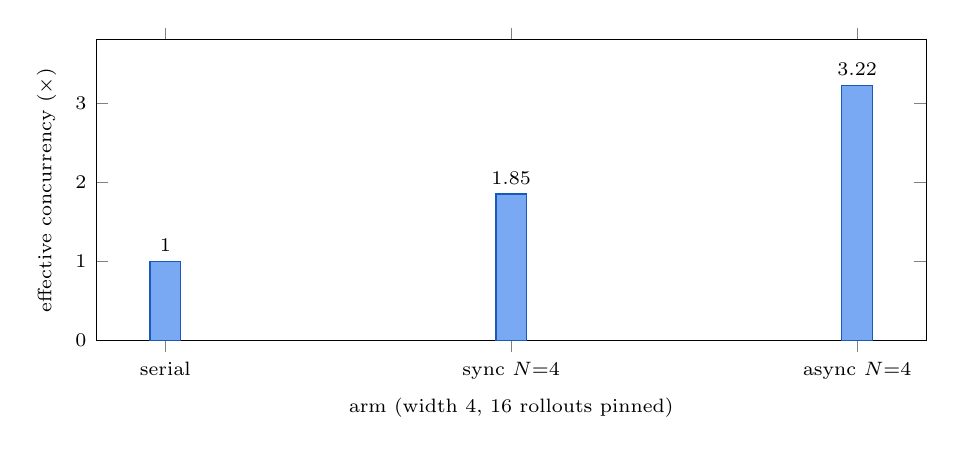
\begin{tikzpicture}
\begin{axis}[
  width=\textwidth, height=5.4cm,
  ybar, bar width=11pt,
  xlabel={arm (width 4, 16 rollouts pinned)},
  ylabel={effective concurrency ($\times$)},
  symbolic x coords={serial, sync $N{=}4$, async $N{=}4$},
  xtick=data, ymin=0, ymax=3.8,
  nodes near coords, nodes near coords style={font=\scriptsize},
  tick label style={font=\scriptsize}, label style={font=\scriptsize},
]
\addplot[fill=adblue!60, draw=adblue!80!black] coordinates {(serial,1.00) (sync $N{=}4$,1.85) (async $N{=}4$,3.22)};
\end{axis}
\end{tikzpicture}
\caption{Effective concurrency (model-seconds $\div$ wall-clock) on the faithful GEPA port, HotpotQA, \code{deepseek-v4-flash}, 16 rollouts pinned on every arm. The serial control is the published loop exactly (one worker, serial gate: overlap $1.00\times$). The round barrier is the whole difference between the parallel arms: the same four workers reach $1.85\times$ with it and $3.22\times$ without it. Wall-clock: 609\,s / 239\,s / 140\,s.}
\label{fig:concurrency}
\end{minipage}\hfill
\begin{minipage}[t]{0.48\textwidth}
\centering
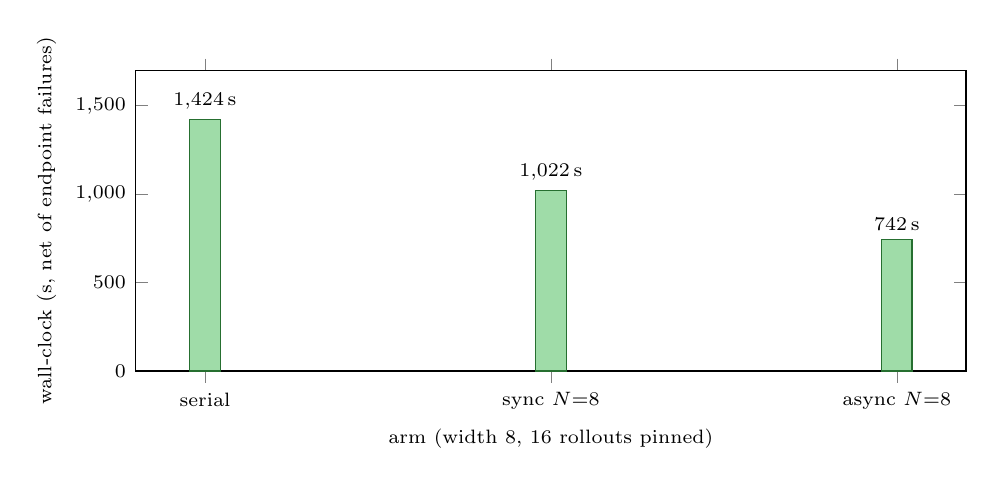
\begin{tikzpicture}
\begin{axis}[
  width=\textwidth, height=5.4cm,
  ybar, bar width=11pt,
  xlabel={arm (width 8, 16 rollouts pinned)},
  ylabel={wall-clock (s, net of endpoint failures)},
  symbolic x coords={serial, sync $N{=}8$, async $N{=}8$},
  xtick=data, ymin=0, ymax=1700,
  nodes near coords={\pgfmathprintnumber{\pgfplotspointmeta}\,s},
  nodes near coords style={font=\scriptsize},
  tick label style={font=\scriptsize}, label style={font=\scriptsize},
]
\addplot[fill=adgreen!50, draw=adgreen!60!black] coordinates {(serial,1424) (sync $N{=}8$,1022) (async $N{=}8$,742)};
\end{axis}
\end{tikzpicture}
\caption{The same comparison at width 8 with GEPA's own Pareto optimizer, \code{GLM-5.2}, wall-clock net of endpoint failures. Model calls: 97 (serial), \textbf{70} (sync --- reflective merge collapses each round's admissions into one sweep, $-28\%$), 95 (async). Raw endpoint probes sustain $7$--$10\times$ concurrency, so the measured ladder ($1.31\times/1.80\times/2.89\times$) is the engine's structure, not the provider's ceiling.}
\label{fig:cost}
\end{minipage}
\end{figure}

We first verify the premise of \cref{sec:concept-parallel}: eight threads over one pool reduce a real \code{GLM-5.2} API workload from 48.6\,s to 8.3\,s ($5.8\times$; sub-linear under heavy-tailed latency), while the same threads on pure-Python CPU work yield $1.1\times$ --- rollout overlap is real and the GIL is not a factor for I/O-bound rollouts.

The main experiment ports GEPA to its own benchmark (HotpotQA \citep{agrawal2025gepa,yang2018hotpotqa}) with 16 rollouts pinned on every arm and a control that reproduces the upstream loop exactly: one worker \emph{and} a serial gate, whose measured overlap is precisely $1.00\times$ (a control that evaluates concurrently is already partially parallel). At width 4 (\cref{fig:concurrency}), the synchronous arm reaches $1.85\times$ effective concurrency and the barrier-free arm reaches $3.22\times$ with the same four workers; wall-clock falls $609 \to 239 \to 140$\,s. At width 8 (\cref{fig:cost}), the two savings of \cref{sec:lever-val} separate cleanly: the synchronous arm realizes merging as a \emph{validation} saving --- 70 model calls versus the serial arm's 97 ($-28\%$), as each round's surviving diffs fuse into a single acceptance test --- while the asynchronous arm realizes the same width as a \emph{wall-clock} saving ($1.92\times$). Model-seconds per rollout fall $37.9 \to 27.7 \to 23.8$ across arms: the parallel arms not only finish sooner but evaluate less, which is the validation-cost reduction observed directly. Endpoint probes sustain $7$--$10\times$ concurrency, so no arm is provider-limited. Two caveats attach to the asynchronous arm: lacking a round boundary, it overran the pinned budget (19 vs.\ 16 rollouts), and at the default lag budget it discarded every stale proposal --- zero-cost at the gate, but paid in proposals.

\subsection{RQ2: Generality across algorithms}
\label{sec:exp-matrix}
To exclude the possibility that the RQ1 result is specific to GEPA, the same scheduler comparison --- serial, synchronous, barrier-free --- is applied to all eleven declarative ports at an equal candidate budget, varying only the scheduler. Paired over $n = 33$ runs, the synchronous-parallel arm outperforms the serial arm by a median $1.36\times$ end-to-end and $1.89\times$ within the engine window, with all eleven methods showing a median improvement. The gap between the two figures is fixed cost outside the engine (dataset retrieval, final test scoring); the gap between $1.89\times$ and the worker count is the barrier and serial gate, i.e.\ precisely what the barrier-free runtime removes in \cref{fig:concurrency}.

\subsection{RQ3: Quality preservation under the aggressive schedule}
\label{sec:exp-ports}

\begin{figure}[t]
\centering
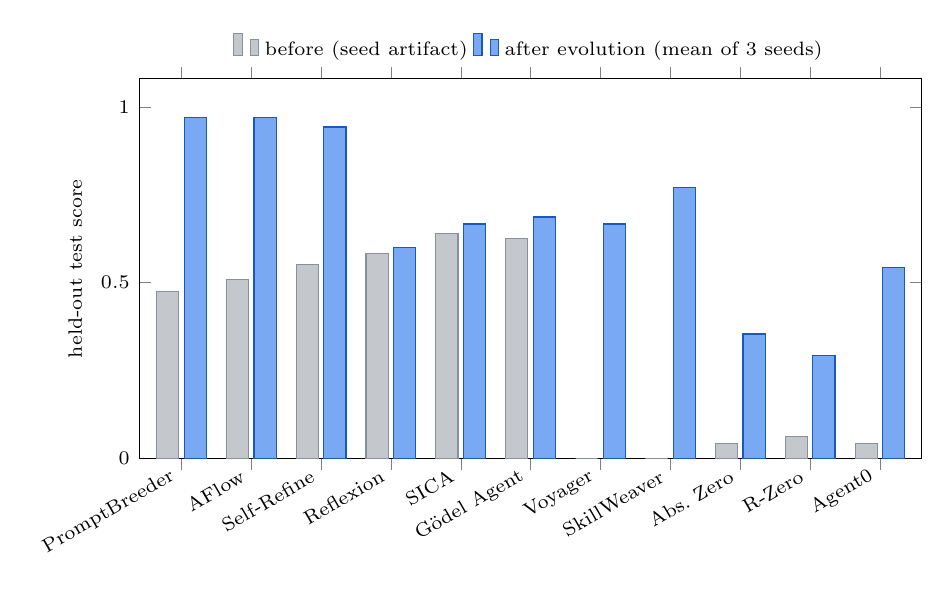
\begin{tikzpicture}
\begin{axis}[
  width=0.95\textwidth, height=6.4cm,
  ybar, bar width=8pt,
  ylabel={held-out test score},
  symbolic x coords={PromptBreeder, AFlow, Self-Refine, Reflexion, SICA, G\"odel Agent, Voyager, SkillWeaver, Abs.\ Zero, R-Zero, Agent0},
  xtick=data, x tick label style={rotate=30, anchor=east, font=\scriptsize},
  ymin=0, ymax=1.08, enlarge x limits=0.06,
  legend style={font=\scriptsize, at={(0.5,1.02)}, anchor=south, legend columns=2, draw=none, fill=none},
  tick label style={font=\scriptsize}, label style={font=\scriptsize},
]
\addplot[fill=adgray!35, draw=adgray!70] coordinates {
  (PromptBreeder,0.474) (AFlow,0.510) (Self-Refine,0.552) (Reflexion,0.583)
  (SICA,0.641) (G\"odel Agent,0.625) (Voyager,0.000) (SkillWeaver,0.000)
  (Abs.\ Zero,0.042) (R-Zero,0.062) (Agent0,0.042)};
\addlegendentry{before (seed artifact)}
\addplot[fill=adblue!60, draw=adblue!80!black] coordinates {
  (PromptBreeder,0.969) (AFlow,0.969) (Self-Refine,0.943) (Reflexion,0.599)
  (SICA,0.667) (G\"odel Agent,0.687) (Voyager,0.667) (SkillWeaver,0.771)
  (Abs.\ Zero,0.354) (R-Zero,0.292) (Agent0,0.542)};
\addlegendentry{after evolution (mean of 3 seeds)}
\end{axis}
\end{tikzpicture}
\caption{Held-out test score before and after evolution for the eleven microports and analogues, each run against \code{deepseek-v4-flash} under the \emph{most aggressive} configuration --- barrier-free async pipeline, 8 workers, Full staleness, 80 rollouts, 3 seeds (465--2{,}069 model calls per seed). All eleven improve. Between 3 and 10 of 240 proposals commit per method --- the acceptance gate admits only strict held-out improvements, so sparse acceptance is the shape of the mechanism, not a low yield. Bars are comparable only within a domain: a gain is bounded by the headroom its baseline leaves.}
\label{fig:eleven}
\end{figure}

Throughput is meaningful only if learning is preserved, so quality is measured under the most aggressive configuration (barrier-free, 8 workers, \textsc{Full} staleness). \Cref{fig:eleven} reports the eleven declarative ports at three seeds each: all improve their held-out test metric, with gains bounded by each benchmark's headroom (the three GSM8K ports converge to 0.94--0.97 and differ in cost rather than quality). Among the benchmark-faithful ports, three representative results: ACE improves FiNER-139 validation $0.719 \to 0.766$ over 120 rollouts while curating a ten-bullet playbook; DGM's best archived child repairs held-out bugs at $0.906$ versus its seed agent's $0.844$ under a frozen \code{pytest} oracle; SkillOpt improves a hard SearchQA subset $0.053 \to 0.211$ with 3 of 43 proposed edits accepted. These single-seed runs establish end-to-end operation, not paper-scale comparisons. The highest-level interface (\code{evolve\_skill}) on 40 HotpotQA rows raises held-out exact match from $0.167$ to $0.583$ over 338 model calls, committing one proposal.

\subsection{RQ4: Merge-of-$N$ versus best-of-$N$ selection at equal budget}
\label{sec:merge-vs-fork}
Throughput cannot distinguish merging from sampling-and-selecting, since $N$ independent forks occupy $N$ workers equally well; the discriminating quantity is held-out quality at an equal rollout budget. The largest such run to date --- HotpotQA on \code{GLM-5.2}, three arms $\times$ three seeds, budget pinned in rollouts, reflective merge enabled so that contradicting proposals survive to fusion; 1{,}298 model calls and 11.3 hours of model time --- yields a \textbf{null result}: merge-of-3 attains the highest median test score together with the widest spread, the intervals overlap, and the framework's own separation test declines to declare a winner. The diagnosis is more informative than the verdict: at this budget the fused union was constructed twice in the entire experiment --- most merges saw a single surviving diff --- so the experiment does not measure a merging deficit; it measures a regime in which merging rarely fired. It also confirms the key-granularity condition of \cref{sec:lever-val} from the opposite direction: without reflective merge, the merge arm on this single-key artifact would have reduced to best-of-$N$ selection. Larger budgets on multi-key artifacts remain the open measurement; the pinned-budget, seeded baseline harness (serial / fork with both oracle and dev-selected reporting / merge) ships with the framework.

\section{Limitations}
\label{sec:limits}

AgentDescent is a research reference implementation. (i) The throughput premise is a testable engineering hypothesis rather than established consensus, and the equal-budget quality question (RQ4) is currently unresolved. (ii) Turn-level checkpoint-and-resume of straggler rollouts and a stratified tail-canary held-out split are designed but not implemented. (iii) Most quality results carry three seeds and the benchmark-faithful ports one; they establish that the mechanisms operate, not effect sizes. Difficulty parameters calibrated on one model did not transfer under a model swap, whereas benchmark-intrinsic difficulty did. (iv) Several earlier project-internal measurements proved irreproducible or favorably defined and were re-measured and corrected in place; every number reported here is generated by a named script. We regard this correction trail as part of the contribution: the evaluation of a self-improving system should satisfy the standard its own acceptance gate imposes on diffs.

\section{Conclusion}
\label{sec:conclusion}

The distributed-training stack admits a coherent counterpart in agent self-evolution once its necessary disanalogy --- diffs do not add --- is taken seriously and merging is constructed as a discrete-space optimizer. Efficiency decomposes into three sources, of which the distinctive one is reduced validation cost: merging collapses $N$ acceptance tests into one, reflective merge extends the reduction to conflicting proposals, and on live models the resulting ladder reads $1.85\times$ with the barrier, $3.22\times$ without, and $28\%$ fewer model calls against a faithful serial control. Eighteen published algorithms adapt as plug-ins rather than forks. Whether merging also improves quality over best-of-$N$ selection at equal budget remains open; the instruments to resolve it ship with the framework.

\section*{Acknowledgments}
The algorithm ports were contributed by \code{chendanyang} (the seven benchmark-faithful ports) and \code{cyanneko} (OpenEvolve and the eleven microports and analogues).

\section*{Reproducibility}
\sloppy
All code is available at \url{https://github.com/Birfy/agentdescent} (MIT license; \code{pip install agentdescent}; the core engine has no required dependencies). Generating scripts: \code{examples/efficiency.py} (thread overlap), \code{bench/matrix\_run.py} and \code{examples/gepa/} (RQ1), \code{bench/candidate\_methods.py} (RQ2, RQ3), \code{bench/baselines\_run.py} (RQ4). Every port supports \code{-{}-dry-run} (no API key or model call) and carries an offline test suite; datasets are retrieved from canonical sources by a dependency-free data layer.

\bibliographystyle{plainnat}
\bibliography{references}

\end{document}
